% !TEX root = ./thesis.tex

\chapter{Technical details}
\label{ch:tede}

This chapter provides technical details relevant to the method proposed in chapter \ref{ch:mode}.
In subsection \ref{ch:nn} we provide an overview of artificial neural networks and related optimization techniques.
Subsection \ref{ch:ae} describes several unsupervised learning techniques for artificial neural networks also known as autoencoders.

\section{Artificial Neural Networks}
\label{ch:nn}
An artificial neural network is a mathematical model inspired by biological brain structure.
A neural network comprises of a set of interacting computational units, called neurons.
In practice, neurons' computation contains a linear transformation of inputs followed by an activation function.
Sigmoid, ReLU and identity functions are among most commonly used activation function.

Neural networks are organized in layers.
A layer can be viewed as a set of neurons that rely on same inputs and have similar behavior i.e. activation function, output size, regularization parameters.
We also distinguish auxiliary layers that perform some transformation of the input data.
Scaling layer, applying nonlinearity function and pooling layer are one of many examples of such layers.

Major neural networks groups are distinguished between each other by structure of connections between neurons.
Feedforward neural networks prohibit cyclic connection and loops in network structure, while Recurrent neural networks have no such restriction.

In subsection \ref{ch:ffnn} we are going to describe basic building blocks of feedforward neural networks.
Subsection \ref{ch:cnn} describes a special case of feedforward neural network with parameter sharing.
Finally, in subsection \ref{ch:opt} we discuss basic concepts of training artificial neural networks.

% \subsection{Artificial Neural Network}
\subsection{Feedforward Neural Networks}
\label{ch:ffnn}

Let's take a look at the simplest case of an artificial neural network: the perceptron.
The single layer perceptron performs a linear transformation of the input values and subsequently applies some activation function $f$:
\begin{equation}\label{eq:per}
  y = f(\sum_{i=1}^N W_ix_i + b) = f(Wx+b)
\end{equation}
where $W$ is a column vector of perceptron parameters and $f$ is an activation function. The structure of the perceptron is depicted in figure \ref{fig:perc}.

% !TEX root = ../thesis.tex

\begin{figure}

\centering
\begin{tikzpicture}
  [
    init/.style={  draw,  circle,  inner sep=2pt,  font=\Huge,  join = by -latex},
    act/.style={  draw,  circle,  inner sep=2pt,  font=\Large,  join = by -latex},
    squa/.style={  draw,  inner sep=2pt,  font=\Large,  join = by -latex},
    start chain=2,node distance=13mm
  ]
  \node[on chain=2] (x2) {$x_2$};
  \node[on chain=2,join=by o-latex] {$w_2$};
  \node[on chain=2,init] (sigma) {$\displaystyle\Sigma$};
  \node[on chain=2,act,label=below:{\parbox{2cm}{\centering Activation \\ function}}] {$f$};
  \node[on chain=2,label=below:Output,join=by -latex] {$y$};
      % {[shift={(0.0,-2.0)}]\centering Activation \\ function}

  \begin{scope}[start chain=4]
  \node[on chain=4] at (0,2.0cm) (b) {$ 1$};
  \node[on chain=4,join=by o-latex] (w0) {$b$};
  \end{scope}

  \begin{scope}[start chain=1]
  \node[on chain=1] at (0,1.0cm) (x1) {$x_1$};
  \node[on chain=1,join=by o-latex] (w1) {$w_1$};
  \end{scope}

  \begin{scope}[start chain=3]
  \node[on chain=3,label=below:Inputs] at (0,-1.5cm) (x3) {$x_n$};
  \node[on chain=3,label=below:Weights,join=by o-latex] (w3) {$w_n$};
  \end{scope}
  % \node[label=above:\parbox{2cm}{\centering Bias \\ $b$}] at (sigma|-w1) (b) {};

  \draw[-latex] (w0) -- (sigma);
  \draw[-latex] (w1) -- (sigma);
  \draw[-latex] (w3) -- (sigma);
  % \draw[o-latex] (b) -- (sigma);

  % \draw[decorate,decoration={brace,mirror}] (x1.north west) -- node[left=10pt] {Inputs} (x3.south west);
  % \draw[decorate,decoration={brace,mirror}] (b.north west) -- node[left=10pt] {Bias} (b.south west);
  \path (x2) -- (x3) node [font=\huge, midway, sloped] {$\dots$};
\end{tikzpicture}
\caption{Structure of a basic computational unit of a neural network (perceptron). Input values $x$ are linearly combined according to the set of parameters $W$ and bias $b$ and activation function $f$ is applied.  }
\label{fig:perc}
\end{figure}


By combining several perceptrons in one set we can produce multiple output values of $y$.
For simplicity, we will stack parameters of $j$ distinct perceptrons that use the same input of size $i$ into matrices $W$ and $b$, where $W$ is rectangular matrix of size $[i,j]$ and $b$ is a column vector of size $j$.
In this case equation $\ref{eq:per}$ remains the same for column vector $y$ of size $j$. A set of perceptron-like neurons that perform computation on the same input forms a single \textit{fully connected} layer of multilayer neural network.

When we combine several layers together we would refer to input vector $x$ as \textit{input layer} and to the last layer of the network producing final output $y$ as \textit{output layer}. All intermediate layers between input and output are called \textit{hidden layers}. We would refer to the depth of the network as to number of computational units on the longest path connecting input and output layers.

It has been shown, that artificial neural network, under mild assumption about the form of the activation function, can act as universal approximator even using a single layer of hidden units of finite size \cite{Debao1993}. Yet, some approximation would require at least exponentially many hidden units in number of inputs $||h||=2^{||x||}$ \cite{Pascanu2014} while using only a single hidden layer. Furthermore, architecutre of $k+1$ layers can be exponentially less complex that architecture of $k$ layers \cite{Bengio2009a}.
Hence, many researchers are developing neural networks with hundreds of layers to allow more compact representations of complex functions \cite{He2015, Srivastava2015}.

Expressivity of the functions that can be approximated by a neural network comes at a cost.
Extensively complex models are prone to overfitting. In other words, models can show excellent performance on the training data while providing poor solutions on yet unseen inputs. In the worst case, an overparameterized model is capable of learning exact mapping between inputs and desired output values without learning useful concepts.

To reduce overfitting several techniques can be used. Reducing model capacity, collecting or generating more training data and regularizing the model are among the most widely used in the context of neural networks.

Using convolutional neural networks is one of the options to reduce capacity of the model by using shared model weights.

% !TEX root = ../thesis.tex

\begin{figure}[t!]
	\centering
	\subfigure[Logistic sigmoid.]{
    		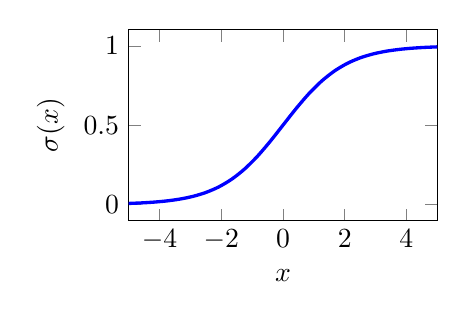
\begin{tikzpicture}
			\begin{axis}[width=5.5cm,height=4cm,ylabel=$\sigma(x)$,xlabel=$x$,ymin=-0.1,ymax=1.1,xmin=-5,xmax=5]
				\addplot[very thick,blue,smooth] {1/(1+exp(-x))};
			\end{axis}
		\end{tikzpicture}
	}
	\subfigure[Hyperbolic tangent.]{
		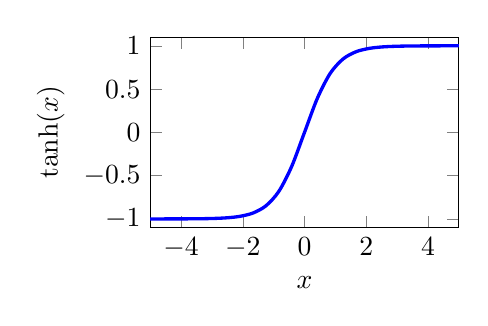
\begin{tikzpicture}
			\begin{axis}[width=5.5cm,height=4cm,ylabel=$\tanh(x)$,xlabel=$x$,ymin=-1.1,ymax=1.1,xmin=-5,xmax=5]
				\addplot[very thick,blue,smooth] {tanh(x)};
			\end{axis}
		\end{tikzpicture}
	}\\
	\subfigure[Rectifier linear unit \cite{Nair2010}.]{
    		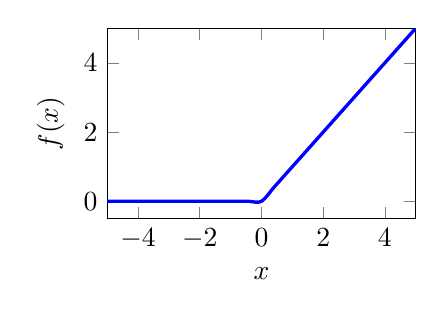
\begin{tikzpicture}
			\begin{axis}[width=5.5cm,height=4cm,ylabel=$f(x)$,xlabel=$x$,ymin=-0.5,ymax=5,xmin=-5,xmax=5]
				\addplot[very thick,blue,smooth] {max(0, x)};
			\end{axis}
		\end{tikzpicture}
	}
	\subfigure[Identity function.]{
		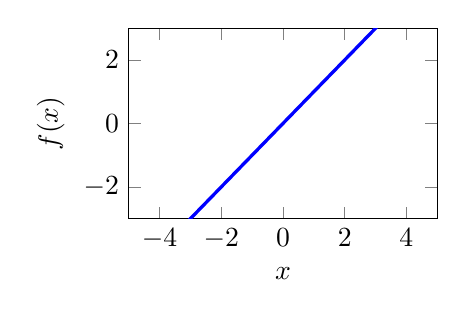
\begin{tikzpicture}
			\begin{axis}[width=5.5cm,height=4cm,ylabel=$f(x)$,xlabel=$x$,ymin=-3,ymax=3,xmin=-5,xmax=5]
				\addplot[very thick,blue,smooth] {x};
			\end{axis}
		\end{tikzpicture}
	}
    	\caption[Sigmoidal activation functions.]{Common choise of activation functions includes logistic sigmoid $\sigma(z)$ and hyperbolic tangent $tanh(z)$. Convolutional neural networks often rely on ReLU and identity functions.}
    	\label{fig:act}
\end{figure}


% \subsection{Artificial Neural Network}
\subsection{Convolutional Neural Networks}
\label{ch:cnn}

The convolutional neural network is a special kind of feedforward neural network that takes advantage of structural organization of the data. This technique allows to decrease the number of parameters of the model when applied to structured data.

Many types of data contain redundant information .i.e. information that, when ignored, can be recovered from the remaining data.
For instance, we can rather easily reconstruct the skipped word in the sentence "\textit{Clouds are in the \_\_}" as well as we can recognize an object on an image when some pixels are altered or missing.
In other words, components of textual or visual data are often interdependent and contain duplicated information.

Convolutional neural networks use small specially adjacent parts of data as neuron inputs. Multiple neurons reuse the same set of parameters $K$, called \textit{kernel}, on distinct patches of the input. All convolutional neurons depending on the same kernel $K$ form a \textit{convolutional filter}. A set of outputs produced by a single convolutional filter is called a \textit{feature map}.



For a 3-dimensional image $I$ of size $H \times W \times C$, where $H$,$W$,$C$ are height, width and number of color channels correspondingly, applying 2-dimensional convolutional filter $K$ of size $w \times h$ would result in a feature map of size $(H-h+1) \times (W-w+1) \times 1$. Kernel $K$ would use $w \times h \times C$ parameters. Convolution operation can be described as:
\begin{equation}\label{eq:conv}
  (I \cdot K)_{x, y} = \sum_a \sum_b \sum_c K_{a,b,c} I_{x+a, y+b,c}
\end{equation}
where ${x, y}$ and ${a,b}$ are two-dimensional indices of feature map and convolution correspondingly and follow next constrains:
\begin{equation*}
  \begin{aligned}
  &1 \leq  x \leq H-h+1, \\
  &1 \leq  y \leq W-w+1, \\
  &1 \leq  a \leq h, \\
  &1 \leq  b \leq w, \\
  &1 \leq  c \leq C.
\end{aligned}
\end{equation*}

\begin{figure}
  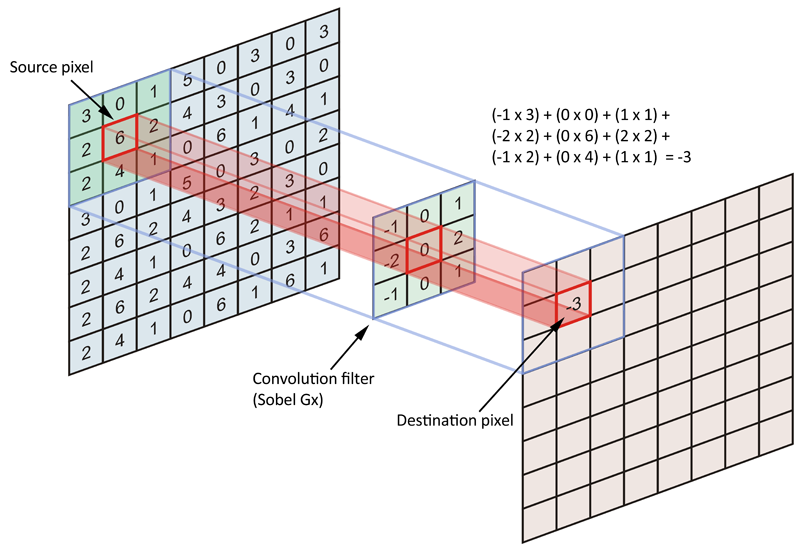
\includegraphics[width=\textwidth,height=\textheight,keepaspectratio]{cnn.png}
  \caption{Illustration of applying convolutional filter of size 3x3 to a single square patch. Output feature map is padded to preserve same shape as input data. Picture taken from [community.arm.com]}
  \label{fig:cnn}
\end{figure}

To preserve width and hight of the feature map $(I \cdot K)$ equivalent to the source image we can add padding along the edges of the input. We can duplicate the same values or use zeros as a padding.
Further, we can apply $k$ distinct convolutional filters to produce output volume of size $x \times y \times k$.

Output of convolution \ref{eq:conv} is often summed with an additional bias $b$ before further processing.
The bias is shared across all convolutional neurons depending on the same kernel.
Value $(I \cdot K)_{x, y}+b$, called \texttt{preactivation}, is forwarded to activation function $\sigma$.

The activation operation can be followed by a pooling operation.
Pooling replaces the output of the convolution layer with summary statistics of nearby outputs.
Max-pooling is one example of such an operation.

\subsubsection{Max-pooling layer}

Max-pooling is a pooling operation applied independently to every feature map.
Max-pooling replaces the output of $\sigma((I \cdot K)_{x, y}+b)$ with a maximum value over a small region of size $w$, $h$ centered at point $(x,y)$.

We can use convolutional and pooling operations in \texttt{strided} mode. When using strides instead of applying operation to every unique position $(x, y)$ we can skip over some indices. Applying strides greater than $1 \times 1$ results in decrease in size of the feature map. For an image of size $H \times W \times C$ and max-pooling operation with stride $h \times w$ we can calculate size of the output feature map as follows $H_o \times W_o \times C $:
\begin{equation*}
  \begin{aligned}
  & W_o = \ceil[\bigg]{\frac{W}{w}} \\
  & H_o = \ceil[\bigg]{\frac{H}{h}} \\
\end{aligned}
\end{equation*}

Downsampling is essential to reduce computational complexity of the network.
Downsampling with pooling layers improves positional tolerance of convolutional networks.
Strided pooling is preferred to strided convolution operation for downsampling. Strided pooling layers are shown to work better in practice, allegedly, due to greater amount of valuable information preserved after downsampling.

Max-pooling operation does not rely on any internal parameters. During training, the position of the maximum element has to be stored. During backpropagation gradients are applied only to the position of the maximum value. Non-maximum elements of the input feature map do not contribute to the total error since they are not used by the upper layers of the network.

\subsection{Network parameters learning}
\label{ch:opt}

TODO: rework with empirical risk minimization in mind. introduce notion of generalization error

Even though a multilayer neural network can approximate large family of compact functions arbitrary well \cite{Debao1993}, finding the right parameters for such approximation is non-trivial.
Lets consider some error function $L(y, f(x, \theta))$ that calculates error between expected values $y$ and the output of the function $f$, realized by a neural network depending on parameters $\theta$. Finding the solution for a general neural network is equivalent to solving next optimization problem:

\begin{equation}\label{eq:optnn}
  \hat{\theta} = \argmin_{\theta \in \Bbb{R}^D} J(\theta) = \argmin_{\theta \in \Bbb{R}^D} \frac{1}{N} \sum_{i=1}^{N} L(y_i, f(x_i, \theta))
\end{equation}
where $D$ is equivalent to number of parameters $||\theta||$ and $N$ is the size of the training set.

Problem \ref{eq:optnn} has no closed-form solution and finding optimal set of parameters $\hat{\theta}$ is an NP-hard problem \cite{Anandkumar16}.
In practice, gradient descent methods are used to find good parametrization $\hat{\theta}$ of the neural network.

Gradient descent methods suggests to iteratively update parameters $\theta_t$ each time taking a step $\eta$ towards the direction of a better solution $\theta_{t+1}=\theta_t - \eta \nabla_\theta \theta$ \cite{Cauchy1847}.
We use vector partial derivatives $\nabla_\theta J(\theta)=\{ \frac{\partial J(\theta)}{\partial w_1}, \ldots, \frac{\partial J(\theta)}{\partial w_N} \}$ of function $J(\theta)$ at point $\theta_t$ as the the direction towards a better solution. Gradient descent method requires both functions $L(y, \hat{y})$ and $f(x, \theta)$ to be differentiable. Note, that differentiability of function $f(x, \theta)$ in $\theta$ implies differentiability of the activation function \ref{eq:per}. Algorithm pseudocode is shown on listing \ref{alg:bp}.

% !TEX root = ../thesis.tex

\begin{algorithm}[H]
 \KwData{X, Y  \text{ (Train set)}}
 \KwResult{$\theta \text{ (Learned weights)}$}

 ${\textbf{Require: } \eta\text{: Stepsize}}$

 $\theta \gets \theta_0 \text{ (Initialization)}$

 \While{not time to terminate}{
  $\triangle_\theta \gets \nabla_\theta J(\theta)(X, Y) \text{ (Calculate gradients)}$

  $\theta \gets \theta - \eta \triangle_\theta\text{ (Update weights)}$

 }

 \Return $\theta$

 \caption{Gradient descent algorithm}\label{alg:bp}

\end{algorithm}


Gradient based methods do not guarantee to find the optimal solution.
Traing can stop in a local minima ($\theta \leq \theta + \eta \delta | \forall \delta \text{ s.t. } |\delta|^2 \leq \epsilon$) or a saddle point.
These cases are shown on figure \ref{fig:critical}.

\begin{figure}[h!]
  \centering
    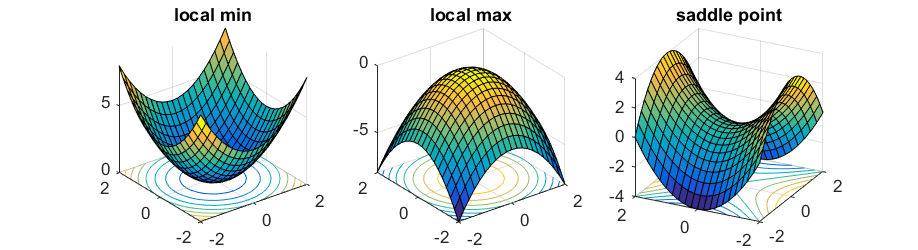
\includegraphics[width=\textwidth,height=\textheight,keepaspectratio]{minmaxsaddle.png}
  \caption{Critical points of a loss function $f(x)$, where $x \in \Bbb{R}^2$.}
  \label{fig:critical}
\end{figure}

In practice, solutions produced by gradient based methods have proven to have satisfying qualities \cite{Szegedy2016,He2015}.
This might be due to the properties of high-dimensional non-convex error surfaces. The study by Y.Dauphin et al. \cite{Dauphin14} concludes, that saddle points and local minima on such surfaces are very likely to be close to global minima.

\subsubsection{Stochastic gradient descent with mini-batches}

Algorithm \ref{alg:bp} requires full path through the complete training set on each iteration.
This might be computationally wasteful for large datasets. Instead, we can perform optimization iteratively only considering subsets of the training set, drawn i.d.d. from the training set:

\begin{equation*}\label{eq:sopt}
  \begin{aligned}
  & \frac{1}{N} \sum_{i=1}^{N} L(y_i, f(x_i, \theta)) = \E_{i \sim U(1,N) } L(y_i, f(x_i, \theta)) \\
  & \E_{i \sim U(1,N) } L(y_i, f(x_i, \theta))= \frac{1}{M} \E_{m \sim U^M(1,N) } \sum_{i \in m} L(y_i, f(x_i, \theta))
  \end{aligned}
\end{equation*}

As a result, we can use the stochastic procedure of selecting $M$ inputs from the training dataset to use in each training iteration.
Subset of inputs selected this way are called \textbf{mini-batches}. Updated algorithm is shown on listing \ref{alg:sbp}.

% !TEX root = ../thesis.tex

\begin{algorithm}[H]
 \KwData{X, Y  \text{ (Train set)}}
 \KwResult{$\theta \text{ (Learned weights)}$}

 $\textbf{Require: } \eta\text{: Stepsize}$

 $\textbf{Require: } M \text{: Minibatch size}$

 $\theta \gets \theta_0 \text{ (Initialization)}$

 \While{not time to terminate}{
  $X_i, Y_i \gets \text{Select $M$ examples i.i.d. from $X, Y$}$

  $\triangle_\theta \gets \nabla_\theta J(\theta)(X_i, Y_i) \text{ (Calculate gradients)}$

  $\theta \gets \theta - \eta \triangle_\theta\text{ (Update weights)}$

 }

 \Return $\theta$

 \caption{Stochastic gradient descent algorithm with minibatches}\label{alg:sbp}

\end{algorithm}


\subsubsection{Backpropagation algorithm}

\subsubsection{Adam update rule}

Training time of gradient descent based algorithm can be reduced by applying adaptive learning rates \cite{Kingma2015}.
\textit{Adam update rule} or simply Adam is one of the algorithms that allow to reduce training time of gradient descent.

The Adam update rule maintains exponential moving average of the gradients $m_t$ and the squared gradient $v_t$.
Hyperparameters $\beta_1, \beta_2$ set the exponential decay rates for both sets of variables.
The update rule for exponential moving average is as follows:
\begin{equation*}
  \begin{aligned}
    & m_t = \beta_1 \cdot m_{t-1} + (1-\beta_1) \cdot g_t \\
    & v_t = \beta_2 \cdot v_{t-1} + (1-\beta_2) \cdot g_t^2
  \end{aligned}
\end{equation*}

Variables $m_t$ and $v_t$ are estimating 1st and 2nd moments of the gradients.
We can therefore rewrite update rule:
\begin{equation}
  \theta_t \gets \theta_{t-1} - \frac{\eta m_t}{\sqrt{v_t} + \epsilon}
\end{equation}
where $\epsilon$ is a small guard value that prevents the divisor from getting too close to zero.

Exponential moving averages $m_t$ and $v_t$ are initialized with zeros.
This leads to zero-bias of the estimators during initial phase of the training.
To accelerate the learning process during first iterations of algorithm \ref{alg:sbp} a time dependent regularization is applied:
\begin{equation*}
  \begin{aligned}
    & \hat{m} = m / (1-\beta_1^t) \\
    & \hat{v} = v/(1-\beta_2^t)
  \end{aligned}
\end{equation*}
where $t$ is a variable tracking current iteration number.

The algorithm requires memory overhead proportional to the number of parameters $||\theta||$. Listing \ref{alg:adam} shows the full algorithm of Adam update rule written in pseudocode.

% !TEX root = ../thesis.tex

\begin{algorithm}[H]
	\KwData{X, Y  \text{ (Train set)}}
	\KwResult{$\theta \text{ (Learned weights)}$}

	$\textbf{Require: } \eta\text{: Stepsize}$

	$\textbf{Require: } \beta_1, \beta_2 \in [0, 1) \text{: Exponential decay rates for the moment estimates}$

	$\textbf{Require: } f(\theta) \text{: Stochastic objective function with parameters } \theta$

	$\textbf{Require: } \theta_0 \text{: Initial parameter vector}$

	$m_0 \gets 0 \text{ (Initialize 1st moment vector)}$

	$v_0 \gets 0 \text{ (Initialize 2nd moment vector)}$

	$t \gets 0 \text{ (Initialize timestep)}$

	\While {$\theta_t$ not converged}{

		$t \gets t + 1$

		$g_t \gets \nabla_\theta f_t(\theta_{t-1}) \text{ (Get gradients w.r.t. stochastic objective at timestep t)}$

		$m_t \gets \beta_1 \cdot m_{t-1} + (1-\beta_1) \cdot g_t \text{ (Update biased first moment estimate)}$

		$v_t \gets \beta_2 \cdot v_{t-1} + (1-\beta_2) \cdot g_t^2 \text{ (Update biased second raw moment estimate)}$

		$\hat{m}_t \gets m_t / (1-\beta_1^t) \text{ (Compute bias-corrected first moment estimate)}$

		$\hat{v}_t \gets v_t/(1-\beta_2^t) \text{ (Compute bias-corrected second raw moment estimate)}$

		$\theta_t \gets \theta_{t-1} - \eta \cdot \hat{m}_t / (\sqrt{\hat{v}_t}+\epsilon) \text{ (Update parameters)}$
	}
	$\textbf{return: } \theta_t \text{ (Resulting parameters)}$

	\caption{Adam, stochastic optimization algorithm. Default settings that work good for tested problems $\eta=0.0001 \ldots 0.001$, $\beta_1=0.9$, $\beta_2=0.999$ and $\epsilon=10^{-8}$} \label{alg:adam}

\end{algorithm}


\subsection{Regularization}

\subsubsection{Bagging}
\subsubsection{Dropout}

Applying an ensemble of models guarantees to perform not worse than any of ensemble members but the computational complexity of the training and evaluation grows linearly with the size of the ensemble. This might play a limiting factor on the size of the ensemble, especially when training of even a single model is computationally expensive.

The \textit{dropout} technique allows to approximately achieve ensemble performance at relatively low computational overhead \cite{Srivastava2014}.
The dropout authors propose to ignore a randomly chosen subset of non-output neurons during training. A new subset of units is selected for each mini-batch or even for each training example.

Training a model with dropout resembles training an ensemble of models. The models automatically follow the same layer structure and share neuron parameters. The number of possible models indirectly trained with dropout is roughly exponential in the number of non-output units $2^{||N||}$. Dropout prohibits only model graphs with broken connection between input and output units. Of course, these models are not trained explicitly and only a small subset is used during the training process. For training with dropout we can update optimization problem \ref{eq:optnn} as follows:

\begin{equation}\label{eq:optnndo}
  \hat{\theta} = \argmin_{\theta \in \Bbb{R}^D} \E_\mu J(\theta, \mu) = \argmin_{\theta \in \Bbb{R}^D} \E_\mu \frac{1}{N} \sum_{i=1}^{N} L(y_i, f(x_i, \theta, \mu))
\end{equation}
where $\mu$ is a random mask.

This way during the training process we minimize the value of $\E_\mu J(\theta, \mu)$ iteratively sampling masks $\mu$ and minimizing function $J(\theta, \mu)$ for this masks explicitly.

To perform prediction with such a model we need to collect votes from an exponential number of ensemble members.
In practice the following two methods are commonly used. First, alike during the training process, we can sample some constant number $N$ of masks $\mu$ and use majority vote on a small subset of functions $\{f(x, \theta, \mu_1), \ldots, f(x, \theta, \mu_N)\}$. Alternatively, it has been shown that simply multiplying the weight of the layers by \textit{keep probability} provides a good approximation of stochastic evaluation \cite{Srivastava2014}. Later method requires only a single forward pass through the complete network for each prediction.

At last, dropout becomes especially useful when it is hard to control the actual model complexity. Developing or even fine-tuning a new task specific neural network architecture is a demanding process. It becomes more common to reuse an existing network architecture as Inception or ResNet \cite{He2015, Szegedy2016}. Even though number of parameters in this networks can be overwhelming for a particular task, rigorous regularization with dropout might be sufficient to achieve satisfactory results.


\section{Autoencoders}\label{ch:ae}
An autoencoder or an autoassociator neural network is an unsupervised learning algorithm that sets target output values equal to input values $y_i=x_i$ \cite{Ng2011,RanzatoMarcAurelio2007}.
Autoencoders are usually trained according to \textit{encoder-decoder} paradigm.
Which first allows to project or encode input $x_i$ into some useful feature representation $h_i$.
Then reconstruct or decode original input $\hat{y_i}$ from representation $h_i$.
This schematically depicted on figure \ref{fig:ae}.


% !TEX root = ../thesis.tex

% \begin{figure}[h!]
%   % \centering
%     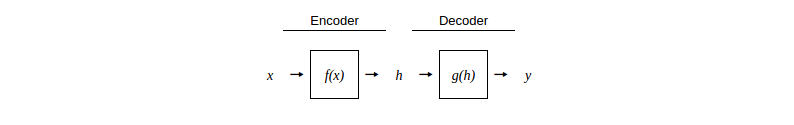
\includegraphics[width=\textwidth,height=\textheight,keepaspectratio]{ae.png}
%   \caption{Autoencoder.}
%   \label{fig:ae}
% \end{figure}


\begin{figure}

\centering
\begin{tikzpicture}
  [
    state/.style={draw, rectangle, minimum width=6mm, minimum height=6mm, inner sep=2pt},
    func/.style={draw, circle, minimum width=1cm, minimum height=1cm, inner sep=2pt},
    loss/.style={draw, diamond, minimum width=1cm, minimum height=1cm, inner sep=2pt},
    node distance=20mm,
    classical/.style={dashed,->,shorten >=4pt,shorten <=4pt,>=stealth}
  ]
  \node (x) [state, label=left:Input] {$x$};
  \node (f) [func, below of=x,label=left:Encoder] {$f(x)$};
  \node(h)[state, below of=f, right of=f,label=below:Features]{$h$};
  \node(g)[func, above of=h, right of=h,label=right:Decoder]{$g(h)$};
  \node(y)[state, above of=g, label=right:Reconstruction]{$y$};
  \node(l)[loss, right of=x, label=below:Loss]{$L2$};

  \draw [->] (x) -- (f);
  \draw [->] (f) -- (h);
  \draw [->] (h) -- (g);
  \draw [->] (g) -- (y);
  \draw [classical] (l) -- (x);
  \draw [classical] (l) -- (y);
\end{tikzpicture}
\caption{An autoencoder with euclidian reconstruction loss.}
\label{fig:ae}
\end{figure}



We are going to refer to encoder as a deterministic differentiable function $f(x, \theta_f)$ that for a given set of parameters $\theta_f$ maps input $x\in \Bbb{R}^d$ into representation $h \in \Bbb{R}^{d'}$.
Likewise, decoder is deterministic differentiable function $g(h, \theta_g)$ depending on parameters $\theta_g$ maps $h\in\Bbb{R}^{d'}$ into $y\in \Bbb{R}^d$. We will further avoid specifying parameters $\theta_f$ and $\theta_g$ for simplicity.
Given a loss function $L$, for a dataset $X=\{x_0, ..., x_i\}$ we can define learning objective as follows \cite{Good2016}:

\begin{equation}\label{eq:ae}
\min_{\theta_f, \theta_g}\sum\limits_{x_i \in X}{L(x_i, g(f(x))}
\end{equation}

Learning identity mapping itself is not particularly useful.
Instead we are often interested in reusing only parts of the autoencoder.
For example, parameters of the encoder $\theta_f$ can serve as a good initialization of a discriminative model \cite{Masci2011, Vincent2010, Zhao2015}.
Such initialization results in minor yet coherent improvement of generalization properties of the model.
Variational Autoencoders, on the other hand, reuse decoder as a generator of new training examples \cite{Kingma2013}.
Extracted features $h$ can represent interpretable properties of the input and can be used to adjust this
properties during generation process \cite{Kulkarni2015, Whitney2016}.

Learning useful feature representation is not a trivial task.
One of the common issues with training autoencoders is possibility to learn identity mapping of input data.
Learning identity mapping would result in less informative feature representation of the inputs.
For example, we can represent both encoder and decoder as a linear function and set the size of the feature space so that it exceeds the size of input space $d' > d$.
Then components of autoencoder can both learn simple identity mapping from input space into feature space and wise-versa.
Therefore, it is common to either limit capacity of the feature space to be less than input space or impose additional regularization on extracted features.

Additionally, both encoder and decoder can be represented as arbitrary neural network.
If capacity of any of two networks is hight enough, it would again lead to learning of identity mapping.
On the other hand, if capacity is chosen too low it can hurt the learning process.
For example, low capacity of generator network in Variational Autoencoders can result in mode collapse.

One of the ways to address the problem of overly high capacity of components can be using stacked autoencoders.
In this approach, instead of directly mapping $h=f(x)$ and $y=g(h)$ into desired lower-dimensional space multiple intermediate mappings can be used $h_i=f_i(h_{i-1})$ and $\hat{h}_i=g_{i+1}(h_{i+1})$.
Stacked autoencoder can be trained in layer-wise manner.
In this case first mappings $y=g_0(h_0)$ and $h_0=f_0(x)$ are trained.
Then follows training of mappings $y_1=g_1(h_1)$ and $h_1=f_0(h_0)$ and so forth.
Architecture of stacked autoencoder is shown on figure \ref{fig:sae}
% \ref{fig}

% !TEX root = ../thesis.tex

\begin{figure}

\centering
\begin{tikzpicture}
  [
    state/.style={draw, rectangle, minimum width=6mm, minimum height=6mm, inner sep=2pt},
    func/.style={draw, circle, minimum width=1cm, minimum height=1cm, inner sep=2pt},
    loss/.style={draw, diamond, minimum width=1cm, minimum height=1cm, inner sep=2pt},
    node distance=20mm,
    classical/.style={dashed,->,shorten >=4pt,shorten <=4pt,>=stealth},
%     dotted/.style={dotted,-,shorten >=4pt,shorten <=4pt,>=stealth}
  ]
  \node (x) [state, label=left:Input] {$x$};
  \node (f1) [func, below of=x,label=left:Encoder 1] {$f_1(x)$};
  \node(h1)[state, below of=f1]{$h_1$};
  \node (f2) [func, below of=h1,label=left:Encoder 2] {$f_2(x)$};
  \node (fn) [func, below of=f2,label=left:Encoder $n$] {$f_n(x)$};

  \node(hn)[state, below of=fn, right of=fn,label=left:Features]{$h_n$};

  \node(gn)[func, above of=hn, right of=hn,label=right:Decoder $n$]{$g_n(h)$};
  \node(g2)[func, above of=gn, label=right:Decoder 2]{$g_2(h)$};
  \node(y1)[state, above of=g2]{$\hat{h}_1$};
  \node(g1)[func, above of=y1,label=right:Decoder 1]{$g_1(h)$};
  \node(y)[state, above of=g1, label=right:Reconstruction]{$y$};

  \node(l1)[loss, right of=x, label=below:Loss]{$L2$};
  \node(l2)[loss, right of=h1, label=below:Loss]{$L2_2$};
  \node(lnce)[loss, below of=hn, label=below:Sparsity penalty]{$L_{NCE}$};

  \draw [->] (x) -- (f1);
  \draw [->] (f1) -- (h1);
  \draw [->] (h1) -- (f2);
  \draw [dotted] (f2) -- (fn);
  \draw [->] (fn) -- (hn);
  \draw [->] (hn) -- (gn);
  \draw [dotted] (gn) -- (g2);
  \draw [->] (g2) -- (y1);
  \draw [->] (y1) -- (g1);
  \draw [->] (g1) -- (y);

  \draw [classical] (l1) -- (x);
  \draw [classical] (l1) -- (y);

  \draw [classical] (l2) -- (h1);
  \draw [classical] (l2) -- (y1);

  \draw [classical] (lnce) -- (hn);
\end{tikzpicture}
\caption{Stacked autoencoders with euclidian distance as reconstruction loss and negative log-likelihood penalty to enforce sparsity of the extracted features.}
\label{fig:mlae}
\end{figure}



\subsection{Autoencoders in computer vision}\label{ch:dcae}

In this subsection we discuss unsupervised learning techniques specific to vision tasks.
First, we describe usage of convolutional layers in autoencoders \ref{ch:cae} and data augmentation \ref{ch:denae}.
Subsection \ref{ch:mod_ae} describes possible modifications of learning objective in autoencoders.

Computer vision tasks often have to work with noisy, highly correlated and very high dimensional data. Input size can grow to thousands of features per input example \ref{ILSVRC15}.
Computer vision models have to account for highly nonlinear relation between input features.
Learned concepts have to be highly tolerant to position of the features on the image grid and be capable to work with spatially transformed and noisy data.
This requirements generally lead to increase in model complexity.

In this subsection we discuss the means of increasing generalization properties of complex computer vision models and modification, more specific to autoencoders.

\subsubsection{Denoising autoencoders}\label{ch:denae}

Learning high capacity models is prone to overfitting.
One of the common ways to decrease overfitting and make model learn useful features without actually changing the model is learning on a larger training corpus.

Denoising autoencoder approach \ref{Vincent2010} allows to increase variation in training data by adding random noise to images. We construct input examples by adding random noise to the dataset according to some parameter $alpha$: $\hat{x}=n(x, \alpha)$.
Denoising autoencoder is yet supposed to reconstruct  the original image $L(x, g(f(x)))$.
This approach expects encoded representation to be stable and robust under condition of input corruption.
It also expects that denoising tasks would result in learning useful structure of input distribution.
Denoising autoencoders are reported to allow better generalization, when encoded network is used as initializer for classifier.

\subsubsection{Convolutional autoencoders}\label{ch:cae}

One of the issues commonly encountered in computer vision tasks is spatial correlation of the data.
Neighboring pixels of a single image are rarely fully independent.
Fully-connected networks are ill-fitted for addressing such local correlation of data.
Furthermore, high dimensionality of computer vision data results in over-parametrization of such models and leads to overfitting.
Recent trends are clearly skewed towards convolutional models \cite{He2015, Szegedy2016} that are consistently showing best results in computer vision competitions \cite{ILSVRC15, Zhou2016}.

Convolutional and max pooling layers provide means of dimensionality reduction.
As described in section \ref{ch:cnn}, applying strided convolutions or pooling layers leads to decrease in resolution of the feature map.
Therefore convolutional and max pooling layers are natural candidates for feature extraction in encoder network.

Convolutional networks depend on relatively small number of parameters.
This quality is desirable for learning useful feature mapping since it allows to avoid overfitting and, as a result, learning of identity mapping by the network.
As described in section \ref{ch:cnn}, number of parameters of convolutional layer depends only on kernel size and depth of the feature map.
Number of parameters required by pooling layers is relatively small if not zero and does not depend on the size of the input.

\subsubsection{Deconvolutional layers and input reconstruction}

While convolutional layers are natural for feature extraction in encoder, reconstruction of highly dimensional input requires a different technique.
One approach is to use an inverse-like operation to convolution.
Deconvolution layer, also known as transposed convolution, is one possible approach.

Deconvolutional layers \cite{Zeiler2010} take as an input an image $y$ composed of $K_0$ color channels $y_1, ... , y_{K_0}$.
As a result of deconvolution process we would like obtain $K_1$ feature maps of the same image.
We can represent each channel $c \in [1, \ldots, K_0]$ as $K_1$ channels convolved with feature maps $f_{k,c}$ \ref{eq:conv}:

\begin{equation}\label{eq:de}
  \sum^{K_1}_{k=1}=z^i_k \cdot f_{k,c} = y^i_{k,c}
\end{equation}

where $\cdot$ is a dot product.

Using this equation we would like to find latent feature maps $f_{k,c}$.
Since equation \ref{eq:de} is an under-determined and allows multiple solution.
Therefore a regularization term $z^i_k$ is added to encourage sparsity of the solutions.
With sparsity term we can express the cost function $C$ for input $y_i$:

\begin{equation}\label{eq:dec}
    C(y_i) = \frac{\lambda}{2} \sum^{K_o}_{c=1} ||\sum^{K_1}_{k=1}{z^i_k \cdot f_{k,c} - y^i_{k,c}}||^2_2 + \sum^{K_1}_{k=1}{|z^i_k|^p}
\end{equation}
where we assume mean square error as a reconstruction cost and $p$ as regularization norm.
Constant $\lambda$ balances contributions of the regularization term to the cost function.

Problem \ref{eq:dec} for simplicity can be decomposed into 2 sequential quadratic problems and solved using stochastic gradient descent method seamlessly with backpropagation.

\subsubsection{Unpooling layers}

Like with convolutional layers, applying pooling layers results in change of the shape of the feature map.
In this subsection we describe a method that allows to effectively revert max-pooling layer preserving relative spatial position of extracted features as on original image.

As described in section \ref{ch:cnn} max pooling layer with stride $k$.
Applying this layers allows to reduce size of feature map $k^2$ times while preserving arguable most important information about extracted features.
Max-pooling is crucial for convolutional neural networks for achieving position tolerance.

Inverse operation of max-pooling is not well defined, since maximum value must be placed somewhere inside original volume of size $k^2$. Naively, we can choose an index of a cell index inside projection volume and put maximum values uniformly into cells with that index.
This procedure is depicted on figure \ref{fig:pool}.
However, this approach destroys relative positioning of unpooled features.
In other words, pooling allows higher lever features to recognize a face by presence of a nose and a mouth within neighboring smaller regions, naive unpooling might place both this features into the same region on the image.

\begin{figure}[h!]
  \centering
    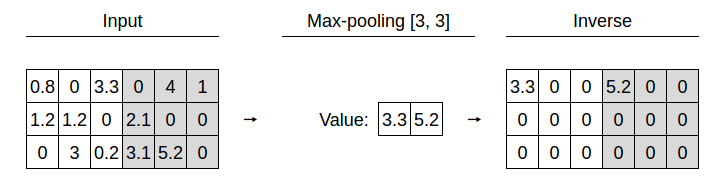
\includegraphics[width=\textwidth,height=\textheight,keepaspectratio]{upsample.png}
  \caption{Upsampling image after max-pooling by placing max value into fixed grid position. Method described by \cite{Dosovitskiy2015a}.}
  \label{fig:pool}
\end{figure}

To address this issue unpooling layer is introduced. Instead of using information about only maximum value of the feature in the region, unpooling layer also uses information about positioning of the feature. This positional information is called a mask. To every pooled value $x_{i,j}$ corresponds a single mask of size equal to pooling region size. To use mask information  unpooling layer take as an input volume with the same shape as produced by pooling layer. As follows, pooling layer describe in section \ref{ch:cnn} must also extract information about position of maximum value. This modification does not otherwise effect the layer neither during forward nor during backward pass. Application of unpooling layer is illustrated on figure \ref{fig:unpool}.

\begin{figure}[h!]
  \centering
    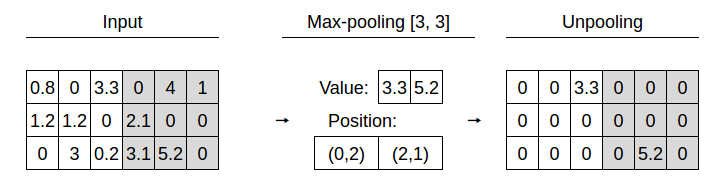
\includegraphics[width=\textwidth,height=\textheight,keepaspectratio]{unpool.png}
  \caption{Illustration of pooling and unpooling layers.}
  \label{fig:unpool}
\end{figure}

Unpooling layers contain no parameters and is not effected by backpropagation.

It worth noting, that mask information extracted by modified pooling layer depends on order of feature channels. As stated by the authors of the original idea, this might have an affect on features, extracted by layers preceding unpooling \cite{Zhao2015}.

\subsubsection{What-Where autoencoders}



\subsection{Extracting useful features with Autoencoders}\label{ch:mod_ae}

Standalone objective \ref{eq:ae} of autoencoder is not particularly useful.
In this section we are going to describe specific use-cases of applying autoencoders along with required modification of objective function.

\subsubsection{Sparse Autoencoders}\label{ch:sae}

Lets consider activations in the hidden layer $h$ for some input $x$:
\begin{equation}
  h(x) = \sigma(W_{h}x_{-1} + b_{h})
\end{equation}
where $W_h$ and $b_h$ are parameters of hidden layer $h$, $x_{-1}$ is output of the previous hidden layer and $\sigma$ is some activation function.
Sparse autoencoders introduce additional term $l_{sparse}$ to loss function to add a constrain on the activations of the hidden layer $h$ \cite{Ng2011}:
\begin{equation}
  l_{total}(x) = l_{reconstruction}(x, g(f(x))) + \alpha*l_{sparse}(x, h(x))
\end{equation}
where $\alpha$ is a constant parameter.

Sparsity constrain tries to achieve low average activation $\hat{\rho}$ on the hidden layer:

\begin{equation}\label{eq:avgh}
  \rho = \frac{1}{N} \sum_{i=1}^N h_i(x)
\end{equation}

For example, lets take a look at the case for sigmoid activation function in the hidden layer.
Sigmoid produces outputs in the interval $[0, 1]$. If we can guarantee average activation on the hidden layer $\hat{\rho} \leq 0.1$ we can rely upon the fact that no more than $10\%$ of hidden neurons would have activation close to $1.0$.

Sparse constrain allows to extract useful features even for relatively high number of hidden units. Specifically, decoder must be able to reconstruct original representation relying only on few high activation on the hidden layer.

There are several ways to enforce sparsity constrain.
It is possible to perform gradient descent directly for fixed value of $\hat{\rho}$. In that case we would have to perform a second pass over the dataset to calculate actual value of $\rho$ to be used as a target during learning with gradient descent. Instead we can simply nullify all but $k$ highest activation during the forward path through the network \cite{Kulkarni2015}.
Or apply negative log-likelihood to the hidden layer of the network \cite{Zhao2015}.
At last, to achieve true zero values on the hidden layer we can use absolute value penalty $l_{sparse}=\sum_{i=1}^N |h_i|$ in conjunction with rectifier linear unit activation function \cite{Glorot2011}.

Sparse coding of the data has proven to be useful to solve classification problem.
In particular, for classification task requires us to assign one of $C$ exclusive classes we can train an autoencoder with $C$ hidden units. Once training converges we expect that features, learned by the hidden layer would somewhat correspond to classes of tasks. We can then use encoder part of the network as initialization of a classifier of the same architecture \cite{Masci2011}.
Such initialization leads to consistently better generalization results after supervised training of the classifier.

\subsubsection{Variational Autoencoders}\label{ch:vae}



% \subsection{Generative adversarial nets}\label{ch:gan}
% \section{Autoencoders and feature interpretability}
